
\section{The history of wakefield acceleration}
Tajima Dawson great Idee, MTV bubble regime, same time PWFA von Rosenzweig... first linear measurements for PWFA
\section{Plasma physics}
There are several definitions of a plasma, but one of the most appealing one that we will follow in this work can be found in the classic 
textbook by Francis F. Chen:
"A plasma is a quasineutral gas of charged and neutral particles which
exhibits collective behavior" \cite{Chen_book_Plasma}.
Regarding the gas types we will conveniently assume them to be electrons, ions and neutral atoms and comment that other particles as well can fit the definition of a plasma, but such exotic compositions are beyond the scope of this work.
\subsection*{Debye Shielding}
The concept of \textit{quasi-neutrality} roots in the shielding behavior of the ions and electrons of charges inside the plasma. 
A positive net charge e.g. originating from a difference in ion density $n_\mathrm{i}$ and electron density $n_\mathrm{e}$ at a temperature $T$
would attract electrons and lead to an electron distribution 
\begin{equation}
f(u) \propto \exp(-\frac{1}{2}\mE v^2+\qE/( k_\mathrm{B}T)).
\end{equation}

With the Poisson Equation 
\begin{align}
\label{eqn:Poisson_plasma}
\epsilon_0 \frac{d^2\Phi}{dx^2}&=-\qE(\nE-n_\mathrm{i})\\
&=\qE \nE (\exp(\qE\Phi/(k_\mathrm{B}T))-1)\\
&\approx \qE\nE(\qE\Phi/(k_\mathrm{B}T)+...)
\end{align}
we can now derive the potential in the plasma
\begin{equation}
\Phi = \Phi_0\exp(-|x|/\lambda_\mathrm{D})
\end{equation}
with the information about the range of the shielded Coulomb field embedded in the Debye Radius
\begin{equation}
\lambda_\mathrm{D}=\sqrt{\frac{\epsilon_0 k_\mathrm{B}T}{n_\mathrm{e}\qE^2}}.
\end{equation}
We can see that a plasma with an edge length $L>>\lambda_\mathrm{D}$ would have its Coulomb fields shielded and appear to an outside observer to be charge-neutral. 



\subsection*{Plasma frequency}
Electrons and ions in a plasma can be described as two fluids, each following the fluid dynamics and interacting via the Maxwell Equations and collisions.

If the electron fluid is displaced with respect to the ion fluid this leads to strong electric fields, acting upon both as a restoring force, but as $m_\mathrm{i}>>\mE$, the electron response is much quicker which is why these kind of plasma oscillations are dominated by the electrons, while the ions can be considered inert.

Starting from equation (\ref{eqn:Poisson_plasma}) with the relation of the electric field and its potential being $\vec{E}=-\nabla \Phi$ 
\begin{equation}
\epsilon_0 \nabla \vec{E}=\qE (n_\mathrm{i}-\nE)
\end{equation}
becomes for small perturbations $n'=\nE+\delta n$
\begin{equation}
\epsilon_0 \nabla \vec{E}=\qE \delta n).
\end{equation}
The solution to this differential equation is a harmonic density oscillation 
\begin{equation}
n(x,t)=\delta n \exp(i(kx-\wP t)).
\end{equation}
The characteristic frequency of this oscillation 
\begin{equation}
\omega_\mathrm{p}=\sqrt{\frac{n_\mathrm{e}q_\mathrm{e}^2}{\epsilon_0 m_\mathrm{e}}}
\end{equation}
is called the \textit{Plasma frequency} and is one of the most important parameters in plasma physics. 
In the field of PWFA it is convenient to also consider the wavelength associated with the plasma oscillations, 
the \textit{Plasma wavelength}
\begin{equation}
\lP=2\pi\frac{\wP}{c}.
\end{equation}

Typical values for example for a plasma density $\nE=1\times10^{17}\mathrm{cm}^{-3}$ are

\begin{align*}
\wP &\approx 56400 \sqrt{\nE [\mathrm{cm}^{-3}]} \approx 1.8\times10^{18}\ 1/s\\
\lP & \approx 105.6 /\sqrt{\nE [10^{17} \mathrm{cm}^{-3} ]} [\mu\mathrm{m}] = 105.6\ \mu\mathrm{m}.
\end{align*} 



It is worth noting that the Debye Shielding assumes a thermalized plasma and is not the right idea of a plasma reaction to a rapid change in charge on a femtosecond timescale. 
The more appropriate figure of merit in that case is the depth an electromagnetic wave with frequency $\omega$ can permeate the plasma fluid given by the skin depth 
\begin{equation}
\kP^{-1}=\frac{c}{\sqrt{\wP^2-\omega^2}}.
\end{equation}

\subsection{time scales}
scattering can be talked about

\subsection{plasma definition}
There are different types of plasmas, but we are only handling with thin, cold  weakly coupled plasmas
\subsection{electromagnetic waves in plasmas}
dispersion relation needs to be talked about. Especially the dispersion relation of lasers during ionization should get some insight here. One has to look into ionization defocussing.  

Wavebreaking limit: \begin{equation}
E_\mathrm{WB}=cm_\mathrm{e}\omega_\mathrm{P}/q_\mathrm{e}\simeq 96 \sqrt{n_\mathrm{e}(\mathrm{cm}^{-3})}
\end{equation}

\subsection{laser ionisation description}
(see diss by Ihar Shchatsinin FU Berlin)

\subsection{Keldysh Parameter}

With $E_{bind}$ being the binding energy and $U_p=\frac{q^2 I}{2 m_e \epsilon_0 c \omega^2}$ being the ponderomotive energy 
\begin{equation}
\gamma=\sqrt{\frac{E_{bind}}{2U_p}}
\end{equation}

$\gamma >1 $ -> Multiphoton Ionisation\\
$\gamma < 1$ tunnel ionisation or BSI

\subsection{ADK theory}
Tunnel ionization is great
	


\subsection{waves in plasmas}
So far everything still flows niocely with working along Chen and Mulser. However now the turn needs to be taken.
The reason is wavebreaking
\subsection{wavebreaking}
Wavebreaking gives us the the ideal way to go from plasma description to blowout description.
\section{PWFA theory}
\subsection{History of PWFA}
A short historic overview is given. 
Maybe mention landau damping? Then of course, Tajima,Dawson. Also MTV and Rosenzweig should be mentioned.
\section{The linear regime}
Herleitung by esarey \cite{RevModPhys.81.1229}


\begin{equation}
E_\xi=4\pi \int_0^\xi \rho{\xi'}\cos(k\mathrm{P}(\xi-\xi'))d\xi
\end{equation}
The transformer ratio $R_\mathrm{trans}=\frac{E_\mathrm{max}^+}{E_\mathrm{max}^-} $ in PWFA is defined as
the ratio of the maximum accelerating electric field
behind the driving bunch, $E_\mathrm{max}^+$, to the maximum decelerating $E_\mathrm{max}^-$
electric field acting upon drive beam electrons. Experimentally the transformer ratio is comparably easy access-able if one assumes the acceleration length for the witness beam and deceleration length for the drive beam to be equal and that the  witness beam is in accelerated at the peak accelerating field.
Then it can be observed in the electron energy spectrum as the maximum energy gain of the witness beam divided by the maximum energy loss of the drive beam. In that sense the transformer ratio is a measure of efficiency with which the drive electron beam can transfer energy to the witness electron beam. 
In the linear regime for a Gaussian drive beam 
In \cite{PhysRevLett.56.1252} it is calculated and simulated that the transformer in the linear regime, which is otherwise limited to $R_\mathrm{trans}\leq 2$ for a symmetric drive beam current profile \cite{bane1984wake}, can reach up to $R_\mathrm{trans}\approx 6.12$ by applying a triangular shaped drive beam current.
\section{The blowout regime}

\section{Descriptions for the blowout regime}
Lotov, Suk, breakdown of fluid theory
Q-tilde and resonant wake excitation.


\section{Accelerator physics}
In the previous chapters we examined the physics of the beam driven plasma wake excitation. 
The ultimate goal as presented in this work is to advantageously make use of the fields in order to inject and accelerate a high quality secondary electron beam, which is conventionally called the witness beam. If there are no substantial advantages between  using the witness over the drive beam for a given application, it might not be worth the effort beyond a scholastic interest.
In this section we will explain the basic electron beam behavior in an accelerator and from that determine the most important parameters. 
\subsection{Single particle movement}

We start with the 
\begin{equation}
\vec{F}=\frac{d\vec{p}}{dt}=q(\vec{E}+\frac{\vec{v}}{c}\times\vec{B})
\end{equation}

Similar to the assumptions made in par-axial optics the electron can be expected to 
follow a straight trajectory in the absence of any deflecting or accelerating force and any small change in that trajectory 
can be expressed in a number of linear changes. 
As in par-axial optics this gives the possibility to describe the electron beam trajectory with linear transformations, represented by a matrix formalism.
This idea can be extrapolated to the entire phase-space information of an electron, so that equation
\begin{equation}
\label{eqn:R_Matrix}
\begin{split}
\Phi_\mathrm{f}&=\hat{R} \Phi_\mathrm{i} \\
\begin{pmatrix}
x_\mathrm{f}\\
x'_\mathrm{f}\\
y_\mathrm{f}\\
y'_\mathrm{f}\\
z_\mathrm{f}\\
\delta_\mathrm{f}\\
\end{pmatrix}
&=
\begin{pmatrix}
R_{11}&R_{12}&R_{13}&R_{14}&R_{15}&R_{16}\\
R_{21}&R_{22}&R_{23}&R_{24}&R_{25}&R_{26}\\
R_{31}&R_{32}&R_{33}&R_{34}&R_{35}&R_{36}\\
R_{41}&R_{42}&R_{43}&R_{44}&R_{45}&R_{46}\\
R_{51}&R_{52}&R_{53}&R_{54}&R_{55}&R_{56}\\
R_{61}&R_{62}&R_{63}&R_{64}&R_{65}&R_{66}\\
\end{pmatrix}
\begin{pmatrix}
x_\mathrm{i}\\
x'_\mathrm{i}\\
y_\mathrm{i}\\
y'_\mathrm{i}\\
z_\mathrm{i}\\
\delta_\mathrm{i}\\
\end{pmatrix}
\end{split}
\end{equation}

describes a complete linear transformation of an electron's phase space vector as a conservative force acts upon it, with the spatial components $x,y,z$, the transverse momenta $x'=\frac{p_\mathrm{x}}{p_\mathrm{z}},y'=\frac{p_\mathrm{y}}{p_\mathrm{z}}$ and the deviation  $\delta=\frac{\delta p_\mathrm{z}}{p_\mathrm{z}}$ from the design momentum $p_\mathrm{z}$
The matrix $\mathbf{R}_\mathrm{m,n}= \frac{\delta \Phi_\mathrm{n}}{\delta \Phi_\mathrm{n}}$ is the Jacobian of this transformation and as that it requires $\mathrm{det}(\hat{R})=1$.


Wiedemann:\cite{Wiedemann_accelerator}


 Jamies book: \cite{Book_Fundamentals_Rosenzweig}
\subsection{Liouville Theorem}
When now considering an entire bunch of electrons it comes in handy to describe it as a smooth phase space distribution
$f(\vec{r},\vec{p})$, which is conventionally normalized so that  
\begin{equation}
\label{eqn:f_int_1}
\int^{\infty}_{-\infty}f(\vec{r},\vec{p})d\vec{r}d\vec{p}=1 .
\end{equation}

The Liouville Theorem states that if only conservative forces are applied to the bunch the total phase volume occupied by the distribution stays constant. This is mathematically equivalent to any transformation that maintains condition (\ref{eqn:f_int_1}), which can be expressed by Jacobian transformations of the kind described by equation (\ref{eqn:R_Matrix}).
Of course $\hat{R}$ does not need to act upon the entire 6D-Phase space. In fact it is common to reduce the analysis and describe only changes in the transverse phase space, the so called \textit{trace space}, as the planes are mathematically independent and often beam-optics that only influence one plane such as quadropoles or dipoles are applied.

In order to obtain a measure of the actual phase space volume the statistical moments of the distribution can be determined by evaluating the integral 
\begin{equation}
<x^n>=\int_{-\infty}^{\infty}f(\vec{r},\vec{p})x^n dx.
\end{equation}
%with the total time differentiate
%\begin{align}
%\frac{d f}{dt}&=\frac{\partial f}{\partial t}+\sum_i \frac{dx_i}{dt}\frac{\partial f}{\partial x_i}+\frac{dp_i}{dt}\frac{\partial f}{\partial p_i}
%&=\frac{\partial f}{\partial t}+\sum_i()
%\end{align}
\subsection{Courant-Snyder coefficients, brightness and emittance}
Courant and Snyder with their summary paper \cite{COURANT1958} have set the standard for defining the phase space volume in the trace space with an ellipse equation for its boundary
\begin{equation}
\label{eqn:CourandSnyderEllipse}
\gamma <x^2>+2\alpha <x> <x'>+\beta <x'^2> =\epsilon.
\end{equation}
\begin{equation}
\alpha =\frac{<x^2>}{\epsilon}, \gamma=\frac{<x'^2>}{\epsilon}, \alpha=\frac{<xx'>}{\epsilon}
\end{equation}
are the so called \textit{Courant Snyder parameters} and $\epsilon$ is the trace space emittance. 
As $f(\vec{r},\vec{p})$ is considered to be smooth function, it might as well consist of a distribution that only approaches 0 so that it is difficult to draw a absolute volume edge as depicted in figure (\ref{img:TraceSpace}).
Because of this and for the sake of simplicity in comparing the value with experimental data, it is useful to work with the rms values. So the \textit{rms trace space emittance} according to \cite{PhysRevSTAB.6.034202} is
\begin{equation}
\epsilon_\mathrm{tr,rms}=\sqrt{<x^2><x'^2>-<xx'>^2}.
\end{equation}
This can additionally be normalized to the \textit{normalized rms trace space emittance} into the form
\begin{equation}
\label{eqn:NormTraceSpaceEmitt}
\epsilon_\mathrm{n,tr,rms}=\frac{p_\mathrm{z}}{\mE c}\sqrt{<x^2><x'^2>-<xx'>^2}
\end{equation} 
so that its value stays current during acceleration.
 
The emittance is an important value, as it is invariant under conservative transformations and therefore an important 
figure of merit for electron beam quality in general. 
Definition (\ref{eqn:NormTraceSpaceEmitt}) will mostly be applied in the context of this work.

\begin{figure}
\label{img:TraceSpace}
\begin{center}
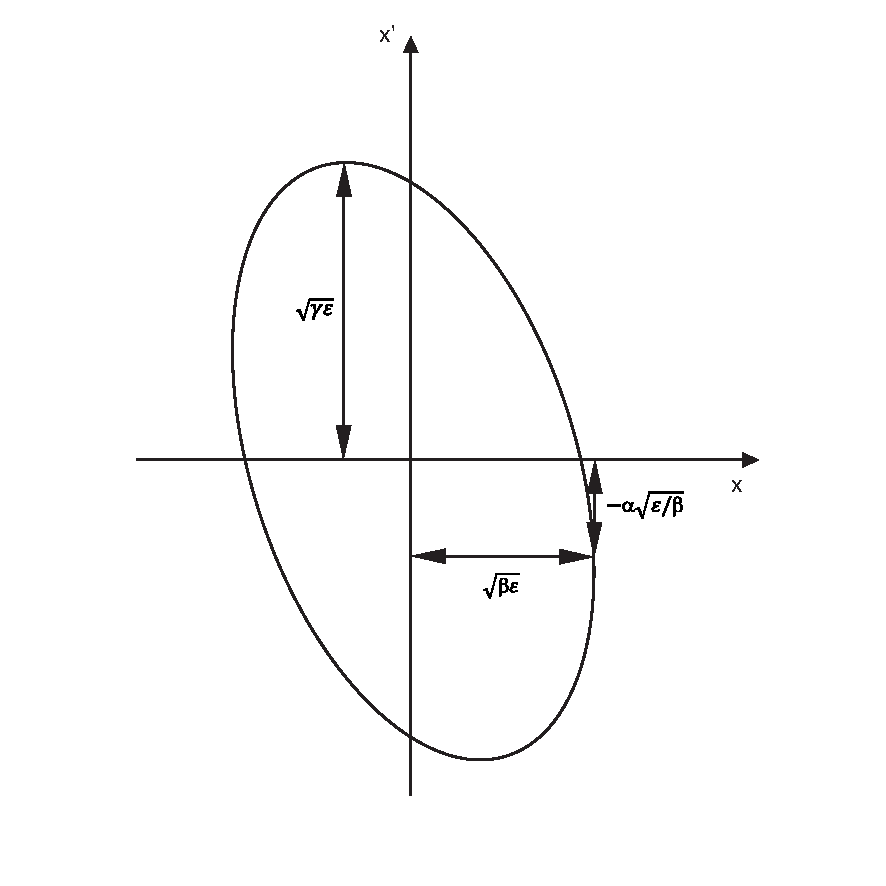
\includegraphics[width=0.6\textwidth]{theory/images/edited/TraceSpaceCourantSnyder.pdf}
\end{center}
\end{figure}
Floettmann 
\subsection{Panowsky-Wenzel Theorem}

original paper:  \cite{Panowsky_Wenzel_original}

 \begin{equation}
W_r =\partial_r W_z
\end{equation} 
This theorem is so important, it clearly needs a subsection. But where ?


\section{Electron Trapping in plasma accelerators}
%The blowout regime inherits an excellent wake field distribution to efficiently accelerate electrons due to the large accelerating fields of the order of $10^{10} \mathrm{V/m}$ and the strong focusing fields in the back of the bubble. Energy can easily be transferred from an driver bunch to a trailing witness electron bunch, which has been sucessfully shown in two-bunch experiments at SLAC. A chirped electron bunch was accelerated to 42 GeV in the linear accelerator, rotated in a magnetic chicane, where the central part of the electron beam was cut out by a collimator and rotated back so that two seperate electron bunches where trailing on the same orbit. In the subsequent plasma stage the wakefields accelerated the witness bunch to up to 84 GeV in only ??? m of acceleration. This external injection scheme was very successfull and has been further studied during the entire experimental period of FACET. With such high fields 
%Even though the fields are DAMN

In order to derive an expression for the trapping condition of a single electron in PWFA, one has to start with the equation of motion for such a single electron. 
\begin{equation}
\vec{F}=\frac{d\vec{p}}{dt}=q(\vec{E}+\frac{\vec{v}}{c}\times\vec{B})
\end{equation}
with the electron charge $q$ electric field $\vec{E}$ and magnetic field $\vec{B}$

This leads to the single particle electron hamiltonian $ H=\gamma m c^2+\Phi$ with the temporal derivative.
\begin{align}
\frac{dH}{dt}&=\frac{d}{dt} (\gamma m_e c^2)+\frac{d}{dt}(q\Phi)\\
&=\vec{v}\frac{d\vec{p}}{dt}+\frac{d}{dt}(q\Phi)\\
&=q\vec{v}(-\nabla \Phi-\frac{\partial \vec{A}}{\partial t})+\frac{\vec{v}\times\vec{B}}{c}+\frac{d}{dt}(q\Phi)\\
&=q(\frac{d}{dt}\Phi-\vec{v}\vec{\nabla}\Phi-\vec{v}\frac{\partial \vec{A}}{\partial t})\\
&=q(\frac{\partial \Phi}{\partial t}-\vec{v}\frac{\partial \vec{A}}{\partial t})
\end{align}

If one assumes now, that the wake fields are constant during the trapping process, then 

\begin{equation}
(\frac{\partial}{\partial t}+v_\mathrm{\phi} \frac{\partial}{\partial z} ) f =   f ( z-v_\mathrm{\phi} t)
\end{equation}\begin{equation}
(\frac{\partial}{\partial t}+v_\mathrm{\phi} \frac{\partial}{\partial z} ) f =0 \ \forall \   f (\vec{r}, z-v_\mathrm{\phi} t)
\end{equation}
which is especially true for the hamiltonian.
\begin{align*}
\frac{d}{dt}H&=q(\frac{\partial \Phi}{\partial t}-\vec{v}\frac{\partial \vec{A}}{\partial t})\\
&=-q v_\mathrm{\phi}(\frac{\partial \Phi}{\partial z}-\vec{v} \frac{\partial \vec{A}}{\partial z}) 
\end{align*}

Since $H-v_\mathrm{\phi}P_z=\mathrm{const.}$

\begin{align}
H-v_\mathrm{\phi}P_z &= \mathrm{const.}\\
\gamma m c^2+\Psi-v_\mathrm{\phi}p_z-v_\mathrm{\phi}qA_z &= \mathrm{const.}\\
\gamma+\frac{q \Phi}{m c^2}-v_\mathrm{\phi} \frac{p_z}{mc^2} &= \mathrm{const.}\\
\gamma - v_\mathrm{\phi} \frac{p_z}{mc^2}- \underbrace{\frac{q}{mc^2}(\Phi-v_\mathrm{\phi}A_z)}_{\bar{\Psi}}  &= \mathrm{const.} 
\end{align}
$\bar{\Psi}$ is the trapping potential, that determines the potential difference for an electron in a potential that moves with a phase velocity $v_\mathrm{\phi}$ with respect to the laboratory frame. It is valid for small as for relativistic velocities.
With the trapping potential one can calculate if an electron inside the plasma wake will be accelerated or not i.e. if electrons will be able to catch up with the wake's velocity during the propagation of the wake or if it will slip out of the potential.
From the prior calculations a general formula can be determined, that compares

\begin{equation}
\label{eq:Trapping_Potential_Pre}
\Delta \bar{\Psi}= \bar{\Psi}_\mathrm{i}-\bar{\Psi}_\mathrm{f}=\gamma_\mathrm{f}-\gamma_\mathrm{i}-\gamma_f\frac{v_\mathrm{\phi}v_\mathrm{f}}{c^2}+\gamma_\mathrm{i}\frac{v_\mathrm{\phi}v_\mathrm{i}}{c^2} 
\end{equation}

In order to honor the name "trapping potential" i.e. to apply this derivation to make predictions of the electron trapping behavior in the plasma wake, it is necessary to define a trapping condition. 
An obvious and conventional choice is that an electron should catch up with the wake's velocity so that 
$v_\mathrm{f}=v_\mathrm{\phi}$.
Equation \ref{eq:Trapping_Potential_Pre} consequently simplifies to 
\begin{equation}
\label{eq:Trapping_Potential_Raw}
\Delta \bar{\Psi}= \gamma_\mathrm{\phi}-\gamma_\mathrm{i}-\gamma_\mathrm{\phi}\frac{v_\mathrm{\phi}^2}{c^2}+\gamma_\mathrm{i}\frac{v_\mathrm{\phi}v_\mathrm{i}}{c^2} 
\end{equation}
Equation \ref{eq:Trapping_Potential_Raw} can be further separated into different physical cases:
\subsection*{luminal wakefield, electron injected  at rest}
In this case the plasma wake travels with a phase velocity near the speed of light, which is the case for beam-driven scenarios with high $\gamma$ driver beams ($v_\mathrm{\phi} \approx c$), and electrons starting inside the wake initially at rest ($v_\mathrm{i} \approx \ 0$).
Here Equation \ref{eq:Trapping_Potential_Raw} simplifies to
\begin{equation}
\Delta \bar{\Psi}=-1
\end{equation}
Examples of this case are the underdense photocathode, or Trojan Horse injection\cite{Hidding_PRL_2012}, or wakefield induced ionization injection\cite{MartinezdelaOssa2014231}.
\subsection*{subluminal wakefield, electron injected at rest}

\begin{equation}
\label{eq:Trapping_Potential_DTH}
\Delta \bar{\Psi}=\gamma_\mathrm{\phi}(1-\frac{v_\mathrm{\phi}^2}{c^2})-1=\gamma_\mathrm{\phi}^{-1}-1
\end{equation}
This formula can for example be applied to ionization injection in LWFA\cite{PakPRL2012} or beam-driven ionization injection schemes in which the wake's phase velocity is retarded such as the Downramp-assisted Trojan Horse (DTH)\cite{DTH}, which this work has as special focus on. In latter case mathematically strictly speaking $\frac{d H}{dt}\neq0 $, but for small changes $\frac{dH}{dt}\approx 0$ during the injection process of the electrons, equation \ref{eq:Trapping_Potential_DTH} can still be applied.
\subsection*{subluminal wakefield, electrons at rest}

\subsection*{superluminal wakefield}
There are physical situations imaginable in which the wake or at least part of the wake move with a phase velocity faster than the speed of light. This is the case for example when a beam driven wake traverses an electron density upramp.
From the previous deductions it seems obvious, that trapping electrons in such a superluminal wakefield is not possible, as $\gamma_\mathrm{\phi}^{-1}$ becomes complex for $v_\mathrm{\phi}>c$.

However, if the superluminosity is only transient as with a short density upramp, the phase velocity will return to $c$ right after the transition. In this case trpping can be possible, but the mathematic tool presented in this section is insufficient to describe the trapping and the phase velocity after the transition is setting the demand on the potential.
\subsection{Trapping position and bunch compression}

Anderson,Serafini:\cite{AndersonVelocBunchPPRSTAB2005,serafini2001velocity}

\subsubsection{emittance preservation}
why don't you ... look at space charge effect to estimate required gamma/acceleration and focusing forces for emittance preservation ? Try looking at Pak's thesis and this emittance paper that claims one needs a fast acceleration, but knows nothing about Trojan Horse yet.
\section{Injection methods in PWFA}
\subsection{Downramp injection}
\subsection{Plasma Torch}
\subsection{Transverse injection ?}
\subsection{ionization injection}
	It could be discussed here how a witness generation might be different for the wake electric fields.
	For example, there is no movement of the release position in xi. But the release won't happen in the potential minimum.
	
\section{Influence of the ionization behaviour}
	Here it is to be described how for TH the co-moving frame is advantagous. dependence of ionization front to 
	create witness beams.
	Image of Ionization front.
	
	
	%\subsection{Rake injection}

\subsection{Trojan Horse injection}
\label{sec:Theory_TrojanHorse}
	
\subsection{Downramp assisted Trojan Horse}

\section{numerical modeling of Trojan Horse injection}

\subsection{Movement of ionization front}
\subsection{emittance growth from space charge}
\subsection{Laser parameter variations}
	
